% Status info:
% M. Gates	2006-2009
% A. Wolf	2011-2014
% B. Gerdes	2013
% Additions inserted from wiki 2015-12-26
% Content OK for 0.12.4.
% 2016-04 GZ started restructuring
% TODO: typo&grammar check

% \chapterimage{chapter-t2-bg} % Chapter heading image now set in guide.tex

\chapter{The User Interface}
\label{ch:gui}


This chapter describes the dialog windows which can be accessed from the left menu bar.

Most of Stellarium's settings can be changed using the view window
(press \guibutton[0.35]{2}{btd_view} or \key{F4}) and the
configuration window (\guibutton[0.35]{2}{btd_config} or
\key{F2}). Most settings have short labels. To learn more about some
settings, more information is available as \emph{tooltips}, small text
boxes which appear when you hover the mouse cursor over a
button.\footnote{Unfortunately, on Windows~7 and later, with NVidia
  and AMD GPUs, these tooltips often do not work.}

\newFeature{0.15} You can drag the
windows around, and the position will be used again when you restart
Stellarium. If this would mean the window is off-screen (because you
start in windowed mode, or with a different screen), the window will
be moved so that at least a part is visible.

Some options are really rarely changed and therefore may only be
configured by editing the configuration file.  See
\ref{sec:ConfigurationFile} The Main Configuration File for more
details.



\section{Setting the Date and Time}
\label{sec:gui:date}

\begin{figure}[h]
\centering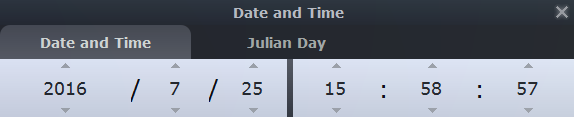
\includegraphics[width=\linewidth]{date_and_time_dialog}
\caption{Date and Time dialog}
\label{fig:gui:date}
\end{figure}

In addition to the time rate control buttons on the main toolbar, you
can use the date and time window (open with the \guibutton[0.35]{2}{btd_time} button or \key{F5}) to set the simulation time. The values
for year, month, day, hour, minutes and seconds may be modified by
typing new values, by clicking the up and down arrows above and below
the values, and by using the mouse wheel.

The other tab in this window allows you to see or set
\indexterm{Julian Day} and/or \indexterm{Modified Julian Day} numbers
(see~\ref{sec:Concepts:JulianDay}).

\section{Setting Your Location}
\label{sec:gui:location}

\begin{figure}[htb]
\centering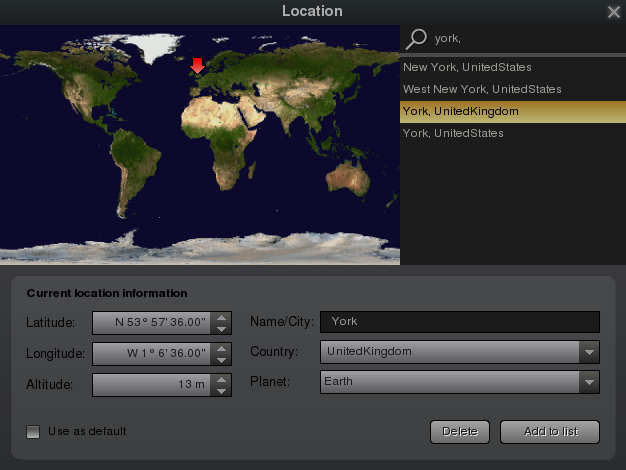
\includegraphics[width=\linewidth]{location_dialog}
\caption{Location window}
\label{fig:gui:location}
\end{figure}

The positions of the stars in the sky is dependent on your location on
Earth (or other planet) as well as the time and date. For Stellarium to
show accurately what is (or will be/was) in the sky, you must tell it
where you are. You only need to do this once -- Stellarium can save your
location so you won't need to set it again until you move.

\newFeature{0.13.1}
After installation, Stellarium uses an online service which tries to
find your approximate location based on the IP address you are
using. This seems very practical, but if you feel this causes privacy
issues, you may want to switch this feature off. You should also consider
switching it off on a computer which does not move, to save network
bandwidth.

To set your location more accurately, or if the lookup service fails,
press \key{F6} to open the location window. There are a few ways you
can set your location:

\begin{enumerate}
\item Just click on the map.
\item Search for a city where you live using the search edit box at
  the top right of the window, and select the right city from the
  list.
\item Click on the map to filter the list of cities in the vicinity of
  your click, then choose from the shortlist.
\item Enter a new location using the longitude, latitude and other
  data.
\end{enumerate}

\noindent If you want to use this location permanently, click on the
``use as default'' checkbox, disable ``Get location from Network'',
and close the location window.



\section{The Configuration Window}
\label{sec:gui:configuration}

The configuration window contains general program settings, and many
other settings which do not concern specific display options. Press
the tool button \guibutton[0.35]{2}{btd_config} or \key{F2} to open.


\subsection{The Main Tab}
\label{sec:gui:configuration:main}


\begin{figure}[bp]
\centering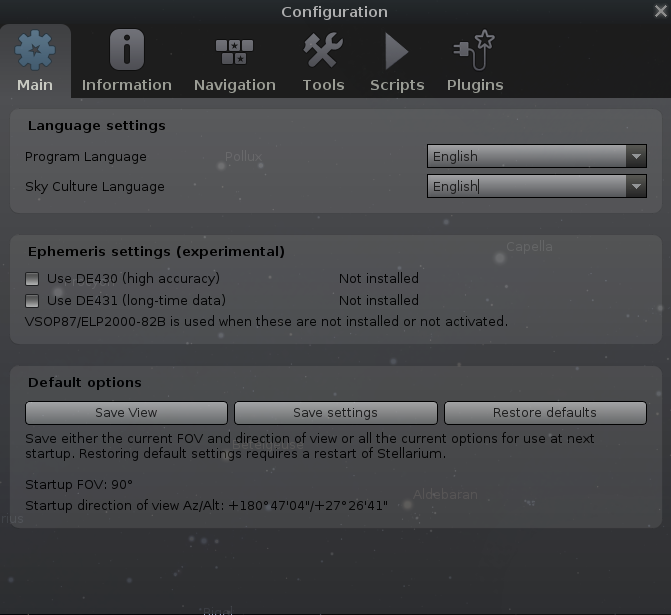
\includegraphics[width=0.65\linewidth]{config_dialog_main_tab}
\caption{Configuration Window: Main Tab}
\label{fig:gui:configuration:main}
\end{figure}

The Main tab in the configuration window provides controls for
changing separately the program and sky culture languages.

The next setting group allows to enable using DE430/DE431 ephemeris
files. Most users do not require this. Thes files have to be installed
separately. See section~\ref{sec:ExtraData:ephemerides} if you are
interested.

The tab also provides a button for saving the current program
configuration. Most display settings have to be explicitly stored to
make a setting change permanent.

\subsection{The Information Tab}
\label{sec:gui:configuration:info}


\begin{figure}[p]
\centering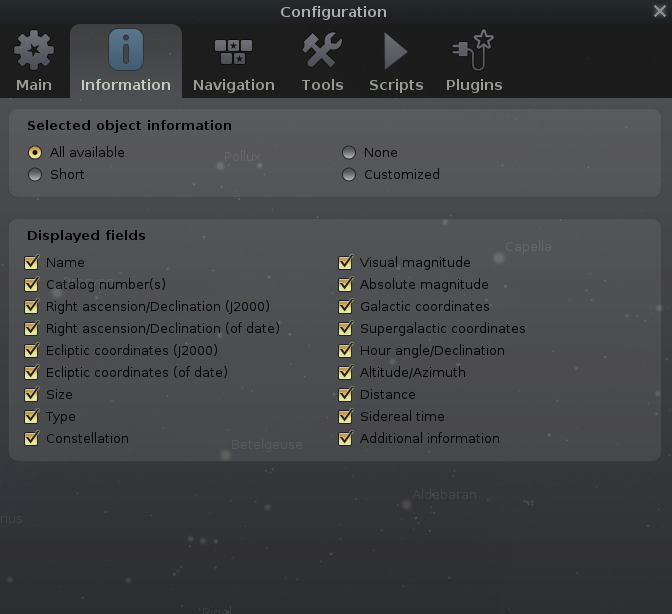
\includegraphics[width=0.65\linewidth]{config_dialog_info_tab}
\caption{Configuration Window: Information Tab}
\label{fig:gui:configuration:info}
\end{figure}

The Information tab allows you to set the type and amount of information
displayed about a selected object.
\begin{itemize}
\item Ticking or unticking the relevant boxes will control this.
\item The information displays in various colours depending on the type and
level of the stored data
\end{itemize}

\subsection{The Navigation Tab}
\label{sec:gui:configuration:nav}


\begin{figure}[p]
\centering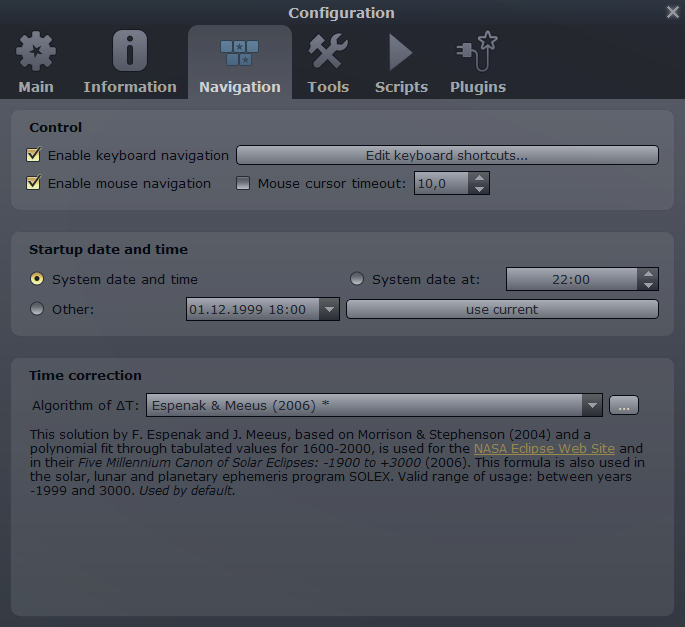
\includegraphics[width=0.65\linewidth]{config_dialog_navigation_tab}
\caption{Configuration Window: Navigation Tab}
\label{fig:gui:configuration:nav}
\end{figure}

The Navigation tab (Fig.~\ref{fig:gui:configuration:nav}) allows for
enabling/disabling of keyboard shortcuts for panning and zooming the
main view, and also how to specify what simulation time should be used
when the program starts:

\begin{description}
\item[System date and time] Stellarium will start with
  the simulation time equal to the operating system clock.
\item[System date at] Stellarium will start with the
  same date as the operating system clock, but the time will be fixed at
  the specified value. This is a useful setting for those people who use
  Stellarium during the day to plan observing sessions for the upcoming
  evening.
\item[Other] some fixed time can be chosen which will
  be used every time Stellarium starts.
\end{description}

The lowest field allows selection of the correction model for the time
correction $\Delta T$ (see section~\ref{sec:Concepts:DeltaT}). Default
is ``Espenak and Meeus (2006)''. Please use other values only if you
know what you are doing.

\subsection{The Tools Tab}
\label{sec:gui:configuration:tools}


\begin{figure}[p]
\centering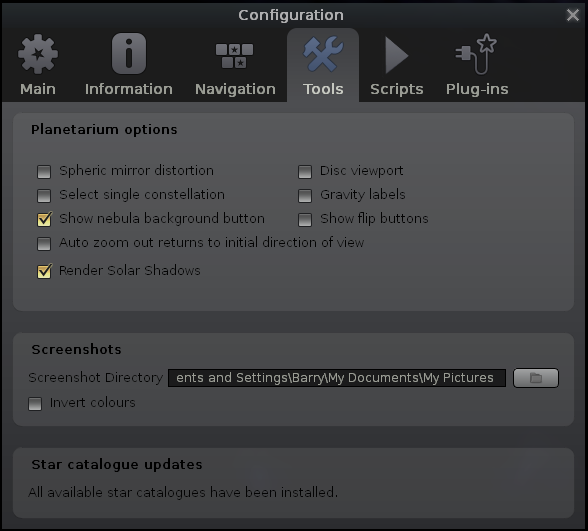
\includegraphics[width=0.65\linewidth]{config_dialog_tools_tab}
\caption{Configuration Window: Tools Tab}
\label{fig:gui:configuration:tools}
\end{figure}

\begin{figure}[p]
\centering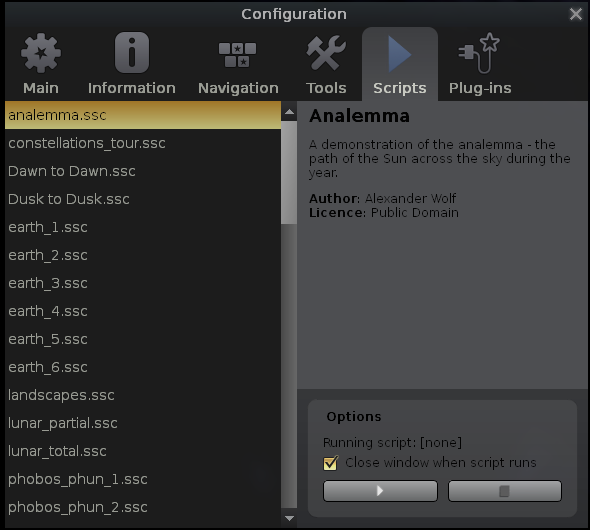
\includegraphics[width=0.65\linewidth]{config_dialog_scripts_tab}
\caption{Configuration Window: Scripts Tab}
\label{fig:gui:configuration:scripts}
\end{figure}

\begin{figure}[p]
\centering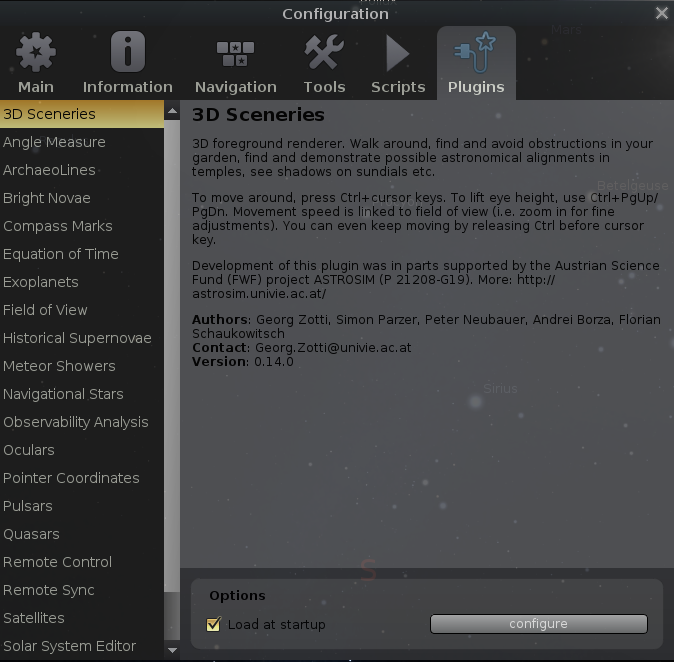
\includegraphics[width=0.65\linewidth]{config_dialog_plugins_tab}
\caption{Configuration Window: Plugins Tab}
\label{fig:gui:plugins}
\end{figure}


The Tools tab (Fig.~\ref{fig:gui:configuration:tools}) contains miscellaneous utility
features:

\begin{description}
\item[Spheric mirror distortion] This option pre-warps the main view
  such that it may be projected onto a spherical mirror using a
  projector. The resulting image will be refected up from the spherical
  mirror in such a way that it may be shone onto a small planetarium
  dome, making a cheap planetarium projection system.
\item[Select single constellation] When active, clicking on a star
  that is member in the constellation lines will make the
  constellation stand out. You can select several constellations, but
  clicking onto a star which is not member of a constellation line
  will display all constellations.
\item[Show nebula background button] You can disable display of DSO
  photographs with this button.
\item[Auto-enabling for the atmosphere] When changing planet during
  location change, atmosphere will be switched as required.
\item[Include nutation] Compute the slight wobble of earth's
  axis. This feature is active only about 500 years around J2000.0.
\item[Azimuth from South] Some users may be used to counting azimuth
  from south.
\item[Disc viewport] This option masks the main view
  producing the effect of a telescope eyepiece. It is also useful when
  projecting Stellarium's output with a fish-eye lens planetarium
  projector.
\item[Gravity labels] This option makes labels of objects in the
  main view align with the nearest horizon. This means that labels
  projected onto a dome are always aligned properly.
\item[Show flip buttons] When enabled, two buttons will be added to
  the main tool bar which allow the main view to be mirrored in the
  vertical and horizontal directions. This is useful when observing
  through telecopes which may cause the image to be mirrored.
\item[Use decimal degrees]
\item[Topocentric coordinates] If you require planetocentric
  coordinates, you may switch this off. Usually it should be enabled.
\item[Auto select landscapes] When changing the planet in the location
  panel, a fitting landscape panorama will be shown when available.
\item[Auto zoom out returns to initial field of view] When enabled,
  this option changes the behaviour of the zoom out key
  (\textbackslash{}) so that it resets the initial direction of view in
  addition to the field of view.
\end{description}

\subsection{The Scripts Tab}
\label{sec:gui:scripts}


The Scripts tab (Fig.~\ref{fig:gui:configuration:scripts}) allows the
selection of pre-assembled scripts bundled with Stellarium that can be
run (See chapter~\ref{ch:scripting} for an introduction to the
scripting capabilities and language). This list can be expanded by
your own scripts as required. See
section~\ref{sec:FilesAndDirectories:DirectoryStructure} where to
store your own scripts.

When a script is selected it can be run by pressing the arrow button
and stopped with the stop button. With some scripts the stop button is
inhibited until the script is finished. %% TODO: EXPLAIN HOW?

Scripts that use sound or embedded videos will need a version of
Stellarium configured at compile time with multimedia support
enabled. It must be pointed out here that sound or video codecs
available depends on the sound and video capabilities of you computer
platform and may not work.


\subsection{The Plugins Tab }
\label{sec:gui:configuration:plugins}


Plugins (see chapter~\ref{ch:Plugins} for an introduction) can be
enabled here (Fig.~\ref{fig:gui:plugins}) to be loaded the next time
you start Stellarium. When loaded, many plugins allow additional configuration
which is available by pressing the \button{configure} button on this tab.




\section{The View Settings Window}
\label{sec:gui:view}

The View settings window controls many display features of Stellarium
which are not available via the main toolbar.

\subsection{Sky Tab}
\label{sec:gui:view:sky}

\begin{figure}[t]
\centering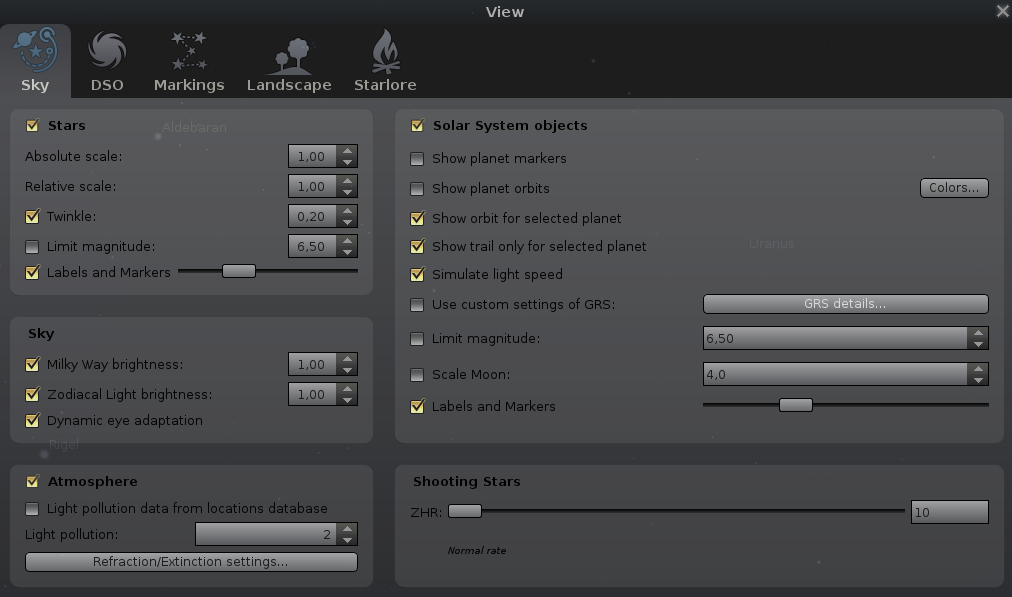
\includegraphics[width=\textwidth]{view_dialog_sky_tab}
\caption{View Settings Window: Sky Tab}
\label{fig:gui:view:sky}
\end{figure}

The Sky tab of the View window (Fig.~\ref{fig:gui:view:sky}) contains settings
for changing the general appearance of the main sky view. Some
hightlights:

\begin{description}
\item[Absolute scale] is the size of stars as rendered by
  Stellarium. If you increase this value, all stars will appear larger
  than before.
\item[Relative scale] determines the difference in size of bright
  stars compared to faint stars. Values higher than 1.00 will make the
  brightest stars appear much larger than they do in the sky. This is
  useful for creating star charts, or when learning the basic
  constellations.
\item[Twinkle] controls how much the stars twinkle when atmosphere is
  enabled. Since V0.15, the twinkling is reduced in higher altitudes,
  where the star light passes the atmosphere in a steeper angle and is
  less distorted.
\item[Limit magnitude] Inhibits automatic addition of fainter stars
  when zooming in. This may be helpful if you are interested in naked
  eye stars only.
\item[Dynamic eye adaptation] When enabled this feature reduces the
  brightness of faint objects when a bright object is in the field of
  view. This simulates how the eye can be dazzled by a bright object
  such as the moon, making it harder to see faint stars and galaxies.
\item[Light pollution] In urban and suburban areas, the sky is
  brightned by terrestrial light pollution reflected in the atmophere.
  Stellarium simulates light pollution and is calibrated to the
  \emph{Bortle Dark Sky Scale} where 1 means a good dark sky, and 9 is
  a very badly light-polluted sky. See Appendix~\ref{ch:BortleScale}
  for more information.
\item[Solar System objects] this group of options lets you turn on
  and off various features related to the planets. Simulation of light
  speed will give more precise positions for planetary bodies which move
  rapidly against backround stars (e.g. the moons of Jupiter). The
  \emph{Scale Moon} option will increase the apparent size of the moon
  in the sky, which can be nice for wide field of view shots.
\item[Labels and markers] you can independantly change the amount of
  labels displayed for planets, stars and nebuulae. The further to the
  right the sliders are set, the more labels you will see. Note that
  more labels will also appear as you zoom in.
\item[Shooting stars] Stellarium has a simple meteor simulation
  option. This setting controls how many shooting stars will be shown.
  Note that shooting stars are only visible when the time rate is 1, and
  might not be visiable at some times of day. Meteor showers are not
  currently simulated.
\end{description}

\subsubsection{Atmosphere settings}
\label{sec:gui:view:sky:atmosphere}

An auxiliary dialog contains detail settings for the atmosphere. Here
you can set atmospheric pressure and temperature which influence
refraction (see section~\ref{sec:phenomena:Refraction}), and the
opacity factor for extinction, \emph{magnitude loss per airmass} $k$
(see section~\ref{sec:phenomena:Extinction}).


\subsection{DSO Tab}
\label{sec:gui:view:dso}

\begin{figure}[t]
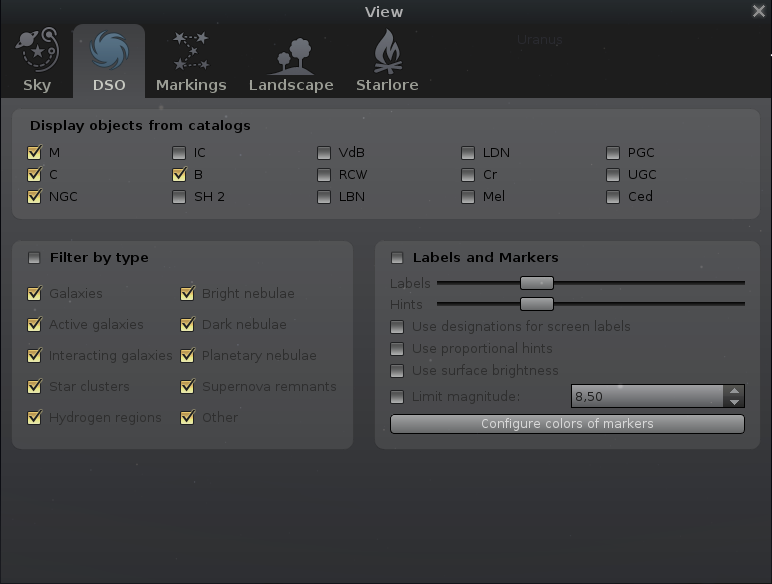
\includegraphics[width=\textwidth,trim=0 70 0 0,clip]{view_dialog_dso_tab}
\caption{View Settings Window: DSO Tab}
\label{fig:gui:view:dso}
\end{figure}


\indexterm{Deep-sky objects} or DSO are extended objects which are
external to the solar system, and are not point-sources like stars.
DSO include galaxies, planetary nebulae and star clusters. These
objects may or may not have images associated with them. Stellarium
comes with a catalogue with over 14,000 extended objects containing
the combined data from many catalogues, with 190 images.  The DSO tab
(Fig.~\ref{fig:gui:view:dso}) allows you to specify which catalogs or
which object types you are interested in. See chapter~\ref{ch:DSO} for
details about the catalog, and how to extend it with your own photographs.





\subsection{Markings Tab}
\label{sec:gui:view:markings}

\begin{figure}[t]
\centering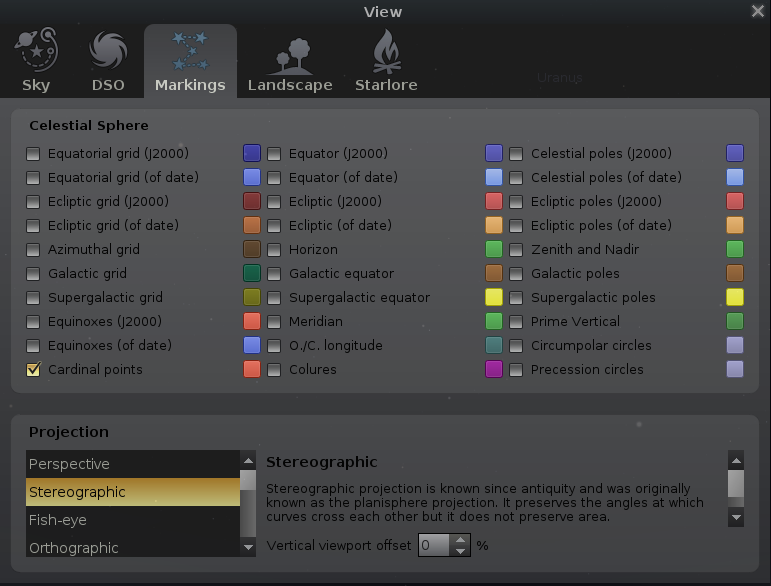
\includegraphics[width=\textwidth]{view_dialog_markings_tab}
\caption{View Settings Window: Markings Tab}
\label{fig:gui:view:markings}
\end{figure}

The Markings tab of the View window
(Fig.~\ref{fig:gui:view:markings}) controls the following features:

\begin{description}
\item[Celestial sphere] this group of options makes it possible to
  plot various grids and lines in the main view.
\item[Projection] Selecting items in this list changes the
  projection method which Stellarium uses to draw the sky~\cite{Snyder:MapProjections}. Options are:

  \begin{description}
  \item[Perspective] Perspective projection maps the horizon and other
    great circles like equator, ecliptic, hour lines, etc. into
    straight lines. The maximum field of view is 150\degree. The
    mathematical name for this projection method is \emph{gnomonic
      projection}.
  \item[Stereographic] Stereographic projection has been known since
    antiquity and was originally known as the planisphere
    projection. It preserves the angles at which curves cross each
    other but it does not preserve area. Else it is similar to
    fish-eye projection mode. The maximum field of view in this mode
    is 235\degree.
  \item[Fish-Eye] Stellarium draws the sky using \emph{azimuthal
    equidistant projection}. In fish-eye projection, straight lines
    become curves when they appear a large angular distance from the
    centre of the field of view (like the distortions seen with very
    wide angle camera lenses). This is more pronounced as the user zooms
    out. The maximum field of view in this mode is 180\degree.
  \item[Orthographic] Orthographic projection is related to
    perspective projection, but the \emph{point of perspective} is set
    to an infinite distance. The maximum field of view is 180\degree.
  \item[Equal Area] The full name of this projection method is
    \emph{Lambert azimuthal equal-area projection}. It preserves the
    area but not the angle. The maximum field of view is 360\degree.
  \item[Hammer-Aitoff] The Hammer projection is an equal-area map
    projection, described by \name{Ernst Hammer} in 1892 and directly inspired
    by the Aitoff projection. The maximum field of view in this mode is
    360\degree.
  \item[Sinusoidal] The sinusoidal projection is a
    \emph{pseudocylindrical equal-area map projection}, sometimes
    called the Sanson--Flamsteed or the Mercator equal-area
    projection. Meridians are mapped to sine curves.
  \item[Mercator] Mercator projection is a cylindrical projection
    which preserves the angles between objects, and the scale around
    an object is the same in all directions. The poles are mapped to
    infinity.  The maximum field of view in this mode is 233\degree.
  \item[Miller cylindrical] The Miller cylindrical projection is a
    modified Mercator projection, proposed by \name{Osborn Maitland Miller}
    (1897--1979) in 1942. The poles are no longer mapped to
    infinity.
  \item[Cylinder] The full name of this simple projection mode is
    \emph{cylindrical equidistant projection} or \emph{Plate
      Carr\'ee}. The maximum field of view in this mode is 233\degree.
  \end{description}
\end{description}

\subsection{Landscape Tab}
\label{sec:gui:view:landscape}

\begin{figure}[t]
\centering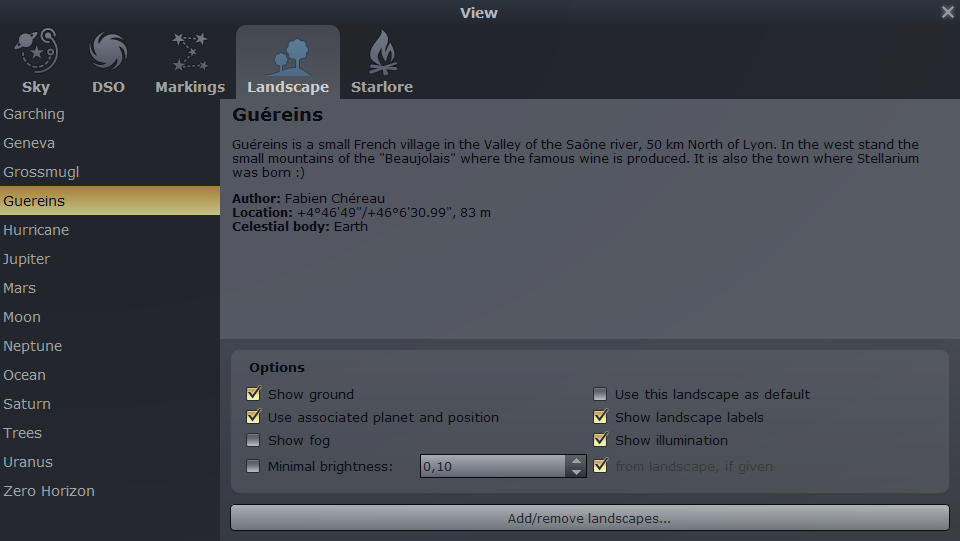
\includegraphics[width=\textwidth]{view_dialog_landscape_tab}
\caption{View Settings Window: Landscape Tab}
\label{fig:gui:view:landscape}
\end{figure}

The Landscape tab of the View window
(Fig.~\ref{fig:gui:view:landscape}) controls the landscape graphics
(the horizon which surrounds you). To change the landscape graphics,
select a landscape from the list on the left side of the window. A
description of the landscape will be shown on the right.

Note that while a landscape  can include information about where the
landscape graphics were taken (planet, longitude, latitude and
altitude), this location does not have to be the same as the location
selected in the Location window, although you can set up Stellarium such
that selection of a new landscape will alter the location for you.

The controls at the bottom right of the window operate as follows:

\begin{description}
\item[Show ground] This turns on and off landscape rendering (same
  as the button \guibutton{0.6}{bt_ground} in the main tool-bar).
\item[Show\_fog] This turns on and off rendering of a band of
  fog/haze along the horizon, when available in this landscape.
\item[Use associated planet and position] When enabled, selecting a
  new landscape will automatically update the observer location.
\item[Use this landscape as default] Selecting this option will save
  the landscape into the program configuration file so that the current
  landscape will be the one used when Stellarium starts.
\item[Minimal brightness] Use some minimal brightness
  setting. Moonless night on very dark locations may appear too dark
  on your screen. You may want to configure some minimal brightness
  here.
\item[from landscape, if given] Landscape authors may decide to
  provide such a minimal brightness value in the \file{landscape.ini}
  file.
\item[Show landscape labels] Landscapes can be configured with a
  gazetteer of interesting points, e.g., mountain peaks, which can be
  labeled with this option.
\item[Show illumination] to reflect the ugly developments of our
  civilisation, landscapes can be configured with a layer of light
  pollution, e.g., streetlamps, bright windows, or the sky glow of a
  nearby city. This layer, if present, will be mixed in when it is
  dark enough.
\end{description}

\noindent Using the button \menu{Add/remove landscapes\ldots}, you can also
install new landscapes from ZIP files which you can download e.g.\
from the Stellarium
website\footnote{\url{http://stellarium.org/wiki/index.php/Landscapes}}
or create yourself (see ch.~\ref{ch:landscapes} Landscapes), or remove
these custom landscapes.

\subsection{Starlore Tab}
\label{sec:gui:view:starlore}

\begin{figure}[t]
\centering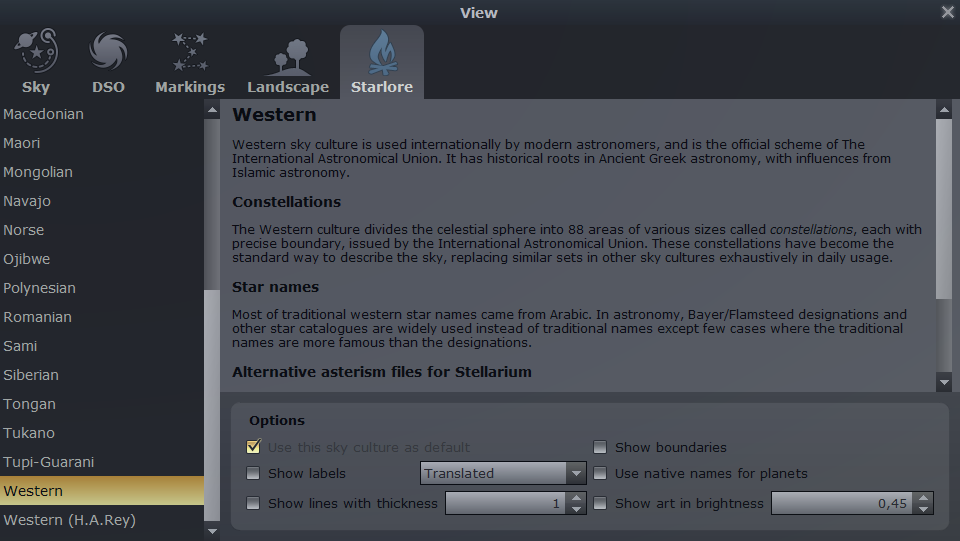
\includegraphics[width=\textwidth]{view_dialog_starlore_tab}
\caption{View Settings Window: Starlore Tab}
\label{fig:gui:view:starlore}
\end{figure}

The Starlore tab of the View window (Fig.~\ref{fig:gui:view:starlore})
controls what culture's constellations and bright star names will be
used in the main display.  Some cultures have constellation art (e.g.,
Western and Inuit), and the rest do not. Configurable options include
\begin{description}
\item[Use this skyculture as default] Activate this option to load
  this skyculture when Stellarium starts.
\item[Show labels] Activate display of constellation labels, like
  \guibutton{0.6}{bt_constellation_name} or \keys{V}. You can further
  select whether you want to display abbreviated, original or
  translated names.
\item[Show lines with thickness\ldots] Activate display of stick
  figures, like \guibutton{0.6}{bt_constellation} or \keys{C}, and you
  can configure line thickness here.
\item[Show boundaries] Activate display of constellation boundaries,
  like \keys{B}. Currently, boundaries have been defined only for
  ``Western'' skycultures.
\item[Use native names for planets] If provided, show the planet names
  as used in this skyculture (also shows modern planet name for
  reference). %% TODO THIS FEATURE NEEDS SOME REWORK!
\item[Show art in brightness\ldots] Activate display of constellation
  art (if available), like \guibutton{0.6}{bt_constellation_art} or
  \keys{R}. You can also select the brightness here.
\end{description}


\section{The Object Search Window}
\label{sec:gui:search}

\begin{figure}[p]
\centering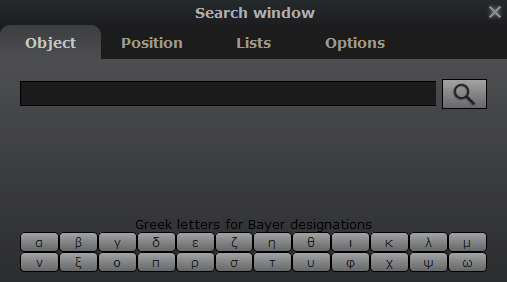
\includegraphics[width=0.7\linewidth]{search_dialog}
\caption{The Search Window: Objects}
\label{fig:gui:search}
\end{figure}

\begin{figure}[p]
\centering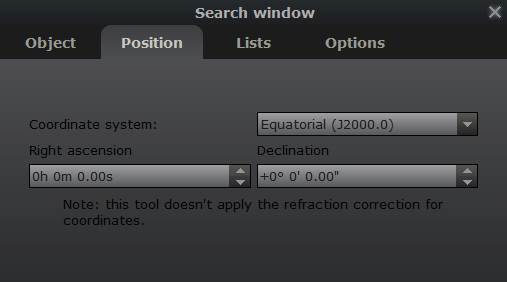
\includegraphics[width=0.7\linewidth]{search_dialog_position}
\caption{The Search Window: Positions}
\label{fig:gui:search:position}
\end{figure}

\begin{figure}[p]
\centering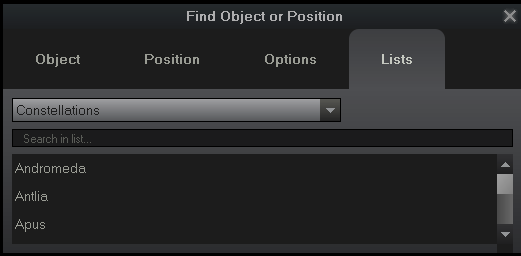
\includegraphics[width=0.7\linewidth]{search_dialog_list}
\caption{The Search Window: Lists}
\label{fig:gui:search:lists}
\end{figure}


\begin{figure}[tp]
\centering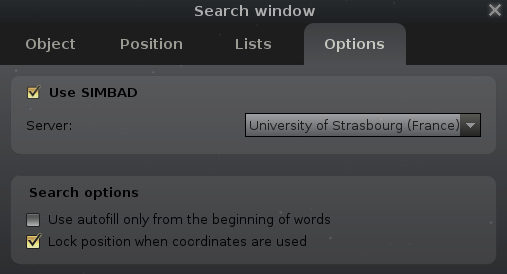
\includegraphics[width=0.7\linewidth]{search_dialog_option}
\caption{The Search Window: Options}
\label{fig:gui:search:options}
\end{figure}

The Object Search window provides a convenient way to locate objects
in the sky. Simply type in the name of an object to find, and press
\key{\return}. Stellarium will point you at that object in the sky.

As you type, Stellarium will make a list of objects which contains 
what you have typed so far. The first of the list of matching objects
will be highlighted. If you press the \key{\tab} key, the selection will change
to the next item in the list. Hitting the \key{\return} key will go to the
currently highlighted object and close the search dialog.

For example, suppose we want to locate Mimas (a moon of Saturn). After
typing the first letter of the name, \emph{m}, Stellarium makes a list
of objects whose name contains M: Haumea, Miranda, Umbriel, \ldots 

You may want at this point to have Stellarium rather propose object
names with start with the string you enter. Do that in the Options tab
of this panel. Now repeat searching (delete, and re-enter M to start
over). Now the list is shorter and contains only objects which start
with M: Maia, Mars, \ldots The first item in this list, Maia, is
highlighted. Pressing \key{\return} now would go to Maia, but we want
Mimas. We can either press \key{\tab} a few times to highlight Mimas
and then hit \key{\return}, or we can continue to type the name until
it is the first/only object in the list.


The Position tab provides a convenient way to enter a set
of coordinates.


The List Search tab allows selection of an object from predefined
sets.  The number of choices is governed by the loaded plug
ins. Simply scroll down the first window to select the type. The name
of an object can then be selected from the list. Press \key{\return} and
Stellarium will go to that object.


The Options tab provides a few settings to fine-tune your search experience.
When the name of an object to find is typed in the object
window and you are connected to the internet and ``Extend search'' is
ticked, Stellarium will search the SIMBAD on-line  data bases for its
coordinates. You can then click the \button{go} button or press return.
Stellarium will point you at that object in the sky even if there is no
object displayed on the screen. The SIMBAD server being used can be
selected from the scroll window.


\section{AstroCalc Window}
\label{sec:gui:AstroCalc}

\newFeature{V0.15} This window provides advanced functionality and is
still in an experimental phase. You can call it by pressing \key{F10}.

% TODO: Add button on left side.


\begin{figure}[htbp]
\centering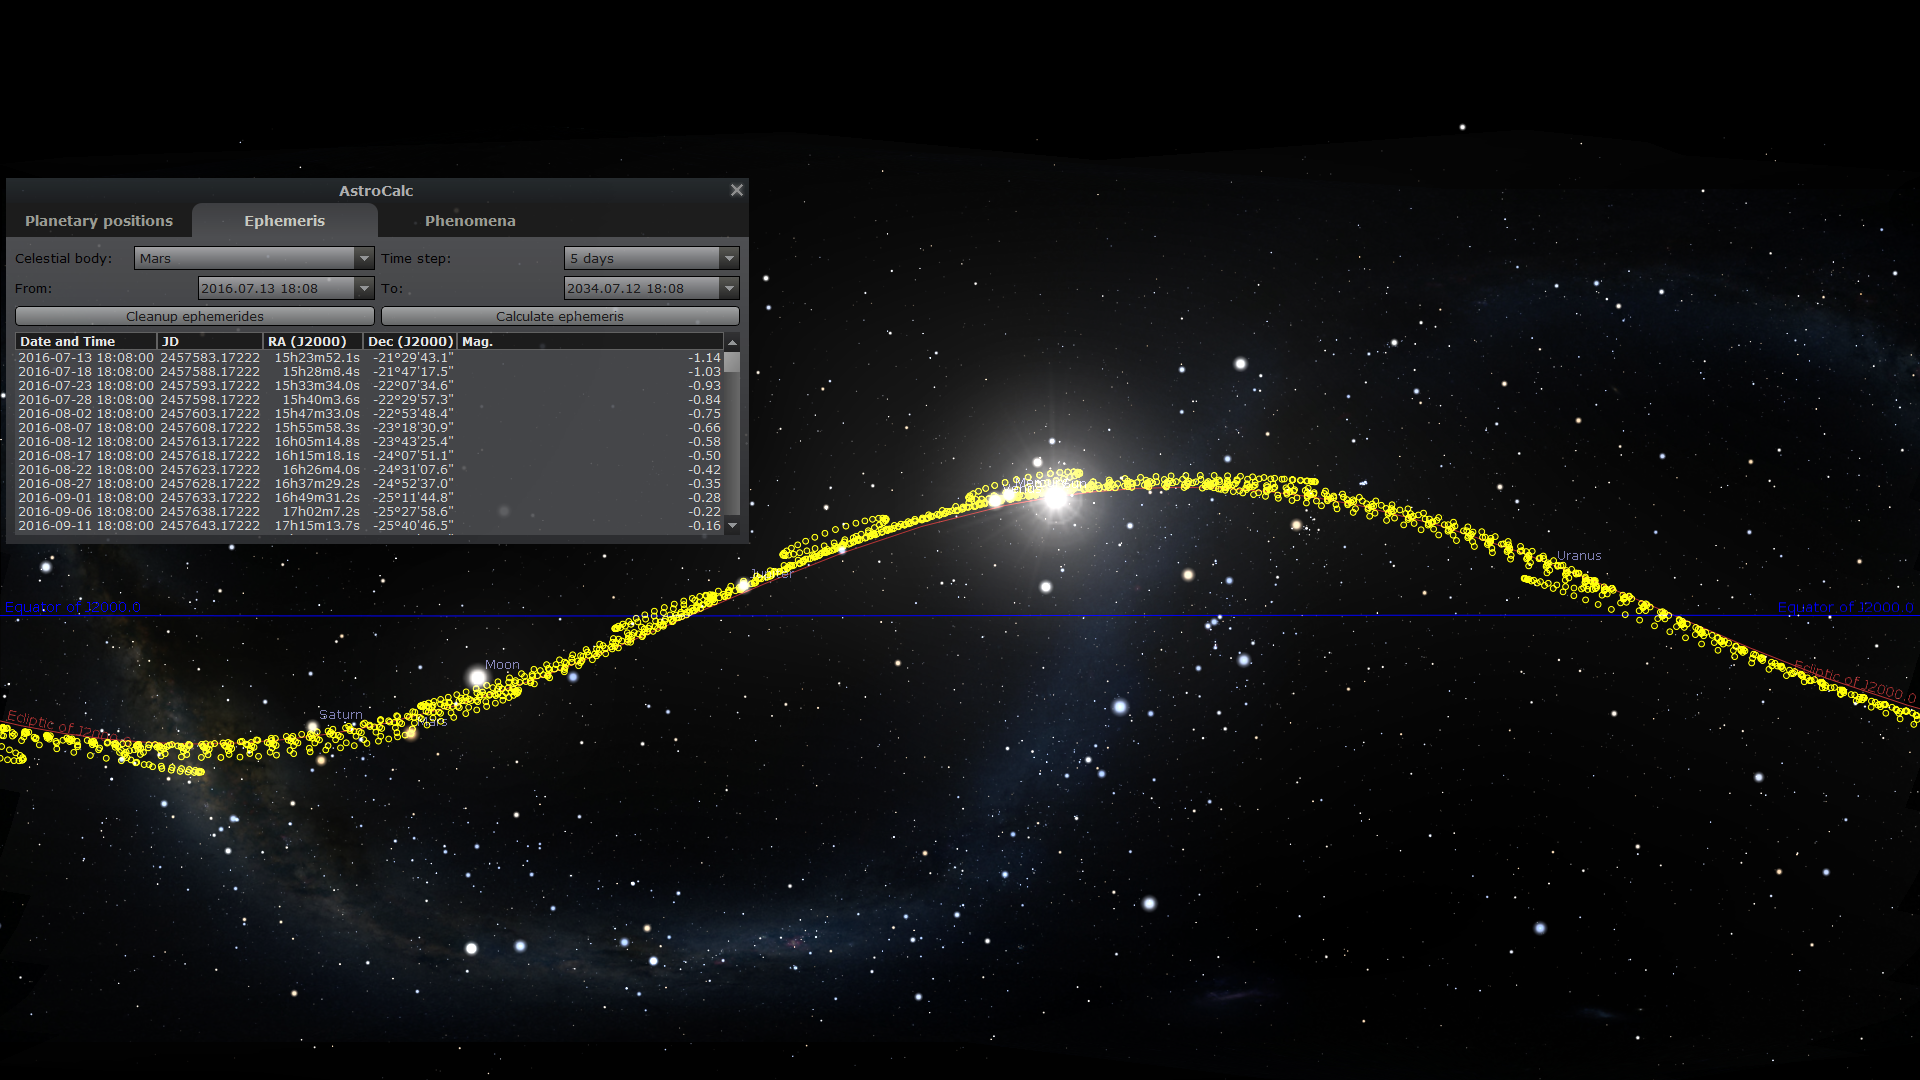
\includegraphics[width=\textwidth]{gui_AstroCalc}
\caption{AstroCalc: Plot traces of planets.}
\label{fig:gui:AstroCalc:Ephemeris}
\end{figure}

\noindent The AstroCalc window shows three tabs with different functionality.
\begin{description}
\item[Planet Positions] Shows J2000.0 positions and magnitudes for all
  installed planets, planet moons, minor bodies (asteroids, comets,
  etc.). Clicking on an entry brings the object into focus.

\item[Ephemeris] Select an object and start and end time, and compute
  an ephemeris (list of positions and magnitude evolving over time)
  for that object. The positions are marked in the sky with yellow
  circles (Figure~\ref{fig:gui:AstroCalc:Ephemeris}). When you click on a date, an orange circle indicates this
  date. Double-clicking sets the respective date and brings object to
  focus. You can export the calculated ephemeris into CSV file. 

\item[Phenomena] Compute phenomena like conjunctions and oppositions
  between planetary objects. You can export the calculated conjunctions and oppositions into CSV file.
\end{description}

\section{Help Window}
\label{sec:gui:help}

\begin{figure}[htbp]
\centering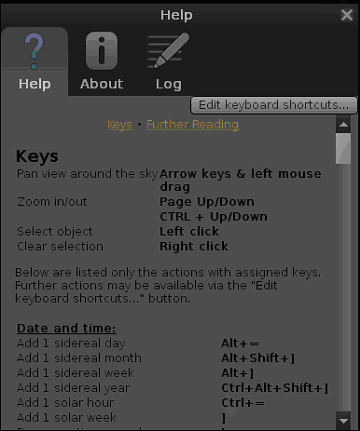
\includegraphics[width=0.7\textwidth]{help_dialog}
\caption{Help Window}
\label{fig:gui:help}
\end{figure}

\noindent The Help window lists all of Stellarium's keystrokes. Note that some
features are only available as keystrokes, so it's a good idea to have
a browse of the information in this window.

\subsection{Editing Keyboard Shortcuts}
\label{sec:gui:help:hotkeys}

You can edit the shortcut keys here. Each available function can be
configured with up to two key combinations. You may want to
reconfigure keys for example if you have a non-English keyboard layout
and some keys either do not work at all, or feel unintuitive for you,
or if you are familiar with other software and want to use the same
hotkeys for similar functions. Simply select the function and click
with the mouse into the edit field, then press your key of choice. If
the key has been taken already, a message will tell you.


\begin{figure}[htbp]
\centering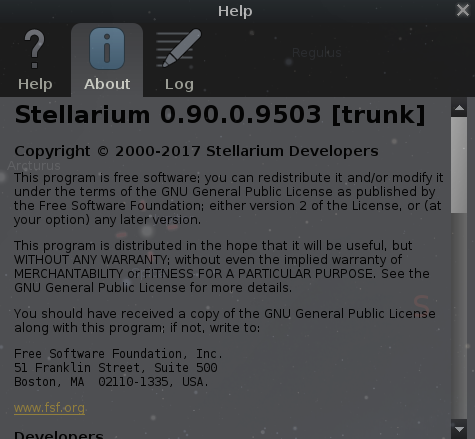
\includegraphics[width=0.68\textwidth]{help_dialog_about}
\caption{Help Window: About}
\label{fig:gui:help:about}
\end{figure}

The About tab (Fig.~\ref{fig:gui:help:about}) shows version and licensing information, and a list
of people who helped to produce the program.

\begin{figure}[htbp]
\centering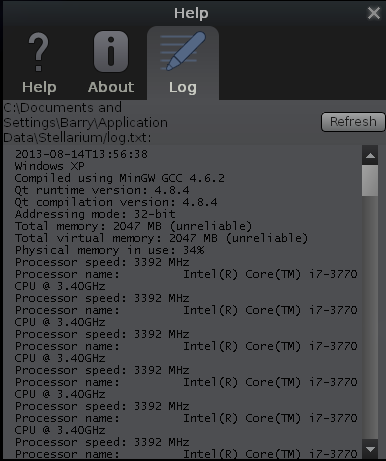
\includegraphics[width=0.68\textwidth]{help_dialog_log}
\caption{Help Window: Logfile}
\label{fig:gui:help:log}
\end{figure}

The log tab (Fig.~\ref{fig:gui:help:log}) shows messages like the loading confirmations carried out when
stellarium runs. It is useful to locate the files that stellarium writes
to your computer. The same information is written to  the file \file{log.txt} that you will
find in your user directory (see~\ref{sec:Directories}).




%%% Local Variables: 
%%% mode: latex
%%% TeX-master: "guide"
%%% End: 
